\section{Battery Models} \label{sec:kibam}
In order to implement the solution, it is necessary to monitor the \gls{soc} and correctly simulate the charging and discharging of the battery. To do this, we need some way of modelling a battery. 
This section will discuss three distinct battery models that all have different qualities. 
An important factor to consider when examining the battery models is the recovery effect, which can have a significant impact on the expected charge lifetime\cite{battery_model}.
The recovery effect charges the battery after a discharge by diffusing the charge evenly in the battery. This means that a battery will regain some charge over time.
The performance of the different models will be compared to actual measurements of a lithium-ion battery, which have been observed by Rakhmatov et al. 2003\cite{battery_lifetime_analysis}, unfortunately we are unable to obtain the specification for the lithium battery used in the paper as they are not listed.
The measurements of the different battery models is the work of Jongerden and Haverkort 2009\cite{battery_model} who used the battery specification and measurements from Rakhmatov et al. 2003\cite{battery_lifetime_analysis}.

The first model, the Ideal model, is simplistic due to it only having two variables to determine the batteries lifetime(L), capacity(C) and load current(I). 
Capacity relates to the battery's amount of amp-hours, and load current is the constant discharge on the battery in amps. 
The calculation for finding the lifetime can be seen in \cref{eq:bm}.
\begin{equation}\label{eq:bm}
L=C/I
\end{equation}

A battery's lifetime under constant and variable load, and the Ideal model's estimate can be seen in \cref{table:t-Ideal}.
The columns ``Meas, min'' hold the actual measured readings of the lithium-ion battery under different loads 
The next column, ``Ideal, min'', holds the Ideal estimation. 
The Ideal model overestimate the expected lifetime in all cases.
It would seem that lower amps with constant loads often results in better predictions than the other tests.
This is not always the case as T5 is better at predicting the lifetime than T6, even though T5 has a higher load.
During variable loads all cases overestimate by a substantial amount, the closest approximation is C5 during variable loads with a 18.5\% overestimation.
The data indicates that the Ideal model does a poor job of estimating the actual lifetime of a battery, which is properly because the model assumes linear effect for lifetime estimation.
Additionally, for variables loads the Ideal model does not consider the recovery effect which further deviate the lifetime from the measured values.
\begin{table}[H]
	\centering
	\scalebox{0.8}{
	\begin{tabular}{|llllll|lllll|}
		\hline
		\multicolumn{6}{|c|}{Constant load} & \multicolumn{5}{c|}{Variable load} \\ \hline
		\rowcolor[HTML]{EFEFEF} 
		\multicolumn{1}{|l|}{\cellcolor[HTML]{EFEFEF}Test} & \multicolumn{1}{l|}{\cellcolor[HTML]{EFEFEF}I, amps} & \multicolumn{1}{l|}{\cellcolor[HTML]{EFEFEF}Meas, min} & \multicolumn{1}{l|}{\cellcolor[HTML]{EFEFEF}Ideal, min} & \multicolumn{1}{l|}{\cellcolor[HTML]{EFEFEF}$\Delta$T} & \%$\Delta$ & \multicolumn{1}{l|}{\cellcolor[HTML]{EFEFEF}Test} & \multicolumn{1}{l|}{\cellcolor[HTML]{EFEFEF}Meas, min} & \multicolumn{1}{l|}{\cellcolor[HTML]{EFEFEF}Ideal, min} & \multicolumn{1}{l|}{\cellcolor[HTML]{EFEFEF}$\Delta$C} & \%$\Delta$ \\ \hline
		T1 & 222.7 & 141.0 & 181.3 & 40.3 & 28.58\% & C1 & 54.5 & 70.8 & 16.3 & 29.91\% \\ \hline
		\rowcolor[HTML]{EFEFEF} 
		T2 & 204.5 & 156.6 & 197.4 & 40.8 & 26.05\% & C2 & 73.3 & 91.9 & 18.6 & 25.38\% \\ \hline
		T3 & 108.3 & 307.8 & 372.8 & 65 & 21.12\% & C3 & 88.3 & 108.5 & 20.2 & 22.88\% \\ \hline
		\rowcolor[HTML]{EFEFEF} 
		T4 & 107.5 & 312.0 & 375.6 & 63.6 & 20.38\% & C4 & 136.0 & 163.0 & 27 & 19.85\% \\ \hline
		T5 & 94.9 & 358.2 & 425.4 & 67.2 & 18.76\% & C5 & 182.7 & 216.5 & 33.8 & 18.50\% \\ \hline
		\rowcolor[HTML]{EFEFEF} 
		T6 & 84.3 & 397.2 & 478.9 & 81.7 & 20.57\% & C6 & 59.0 & 74.7 & 15.7 & 26.61\% \\ \hline
		T7 & 75.5 & 448.2 & 534.8 & 86.6 & 19.32\% & C7 & 51.1 & 66.9 & 15.8 & 30.92\% \\ \hline
		\rowcolor[HTML]{EFEFEF} 
		T8 & 28.0 & 1248 & 1442 & 194 & 15.54\% & C8 & 55.0 & 70.8 & 15.8 & 28.73\% \\ \hline
		T9 & 19.5 & 1818 & 2071 & 253 & 13.92\% & C9 & 54.9 & 70.8 & 15.9 & 28.96\% \\ \hline
		\rowcolor[HTML]{EFEFEF} 
		T10 & 3.0 & 12690 & 13458 & 768 & 6.05\% & C10 & 142.7 & 171.3 & 28.6 & 20.04\% \\ \hline
	\end{tabular}}
	\caption{Comparison of actual measurements and predictions from the Ideal model. The specification for the variable loads can be found in \cref{table:variable_loads_list}.}
	\label{table:t-Ideal}
\end{table}

The next model, Peukert Model, introduces a few new variables in comparison to the Ideal model. 
To better represent the battery, a non-linear model is needed as it is naive to represent it linearly.
To do so, Peukert updates the formula to what can be seen in \cref{eq:pm}. 
\begin{equation}\label{eq:pm}
L=(\frac{C}{I^k})
\end{equation}
\begin{itemize}
	\item L - lifetime in hours
	\item C - capacity in AH
	\item I - load current in amps
	\item k - Peukert Exponent
\end{itemize}

According to Martin 1999\cite{peu} C is the battery's capacity and k is a value that often lies between 1.2 and 1.7.
This equation describes the lifetime for constant loads.
It can be hard to determine the exact value of k without actual testing the battery, but it is sometimes provided by the manufacturers in their data sheets.

\Cref{table:t-Peukert} showcases the estimates using Peukert. In most cases Peukert overestimate, except for one instance in test T10 where it underestimate with 3.17\%.
Peukert seems to become more accurate with smaller amps, alike to how the Ideal model behaved.
However, it still has a high mismatch compared to measured values with variable loads, this is due to Peukert's model is not taking the recovery effect into account.
\begin{table}[H]
	\centering
	\scalebox{0.8}{
	\begin{tabular}{|llllll|lllll|}
\hline
\multicolumn{6}{|c|}{Constant load} & \multicolumn{5}{c|}{Variable load} \\ \hline
\rowcolor[HTML]{EFEFEF} 
\multicolumn{1}{|l|}{\cellcolor[HTML]{EFEFEF}Test} & \multicolumn{1}{l|}{\cellcolor[HTML]{EFEFEF}I, amps} & \multicolumn{1}{l|}{\cellcolor[HTML]{EFEFEF}Meas, min} & \multicolumn{1}{l|}{\cellcolor[HTML]{EFEFEF}Peukert, min} & \multicolumn{1}{l|}{\cellcolor[HTML]{EFEFEF}$\Delta$T} & \%$\Delta$ & \multicolumn{1}{l|}{\cellcolor[HTML]{EFEFEF}Test} & \multicolumn{1}{l|}{\cellcolor[HTML]{EFEFEF}Meas, min} & \multicolumn{1}{l|}{\cellcolor[HTML]{EFEFEF}Peukert, min} & \multicolumn{1}{l|}{\cellcolor[HTML]{EFEFEF}$\Delta$C} & \%$\Delta$ \\ \hline
T1 & 222.7 & 141.0 & 154.5 & 13.5 & 9.57\% & C1 & 54.5 & 60.5 & 6 & 11.01\% \\ \hline
\rowcolor[HTML]{EFEFEF} 
T2 & 204.5 & 156.6 & 168.4 & 11.8 & 7.54\% & C2 & 73.3 & 79.1 & 5.8 & 7.91\% \\ \hline
T3 & 108.3 & 307.8 & 321.3 & 13.5 & 4.39\% & C3 & 88.3 & 93.8 & 5.5 & 6.23\% \\ \hline
\rowcolor[HTML]{EFEFEF} 
T4 & 107.5 & 312.0 & 323.7 & 11.7 & 3.75\% & C4 & 136.0 & 142.5 & 6.5 & 4.78\% \\ \hline
T5 & 94.9 & 358.2 & 367.5 & 9.3 & 2.60\% & C5 & 182.7 & 190.2 & 7.5 & 4.11\% \\ \hline
\rowcolor[HTML]{EFEFEF} 
T6 & 84.3 & 397.2 & 414.4 & 17.2 & 4.33\% & C6 & 59.0 & 64.4 & 5.4 & 9.15\% \\ \hline
T7 & 75.5 & 448.2 & 463.6 & 15.4 & 3.44\% & C7 & 51.1 & 56.5 & 5.4 & 10.57\% \\ \hline
\rowcolor[HTML]{EFEFEF} 
T8 & 28.0 & 1248 & 1270 & 22 & 1.76\% & C8 & 55.0 & 60.5 & 5.5 & 10.00\% \\ \hline
T9 & 19.5 & 1818 & 1835 & 17 & 0.94\% & C9 & 54.9 & 60.5 & 5.6 & 10.20\% \\ \hline
\rowcolor[HTML]{EFEFEF} 
T10 & 3.0 & 12690 & 12288 & -402 & -3.17\% & C10 & 142.7 & 148.8 & 6.1 & 4.27\% \\ \hline
\end{tabular}}
	\caption{Comparison of actual measurements and predictions from the Peukert model. The specification for the variable loads can be found in \cref{table:variable_loads_list}.}
	\label{table:t-Peukert}
\end{table}

The \gls{kibam} uses two wells as an abstract concept for representing a battery.
It consist of an available and a bound charge as shown in \cref{fig:kibam_wells}.
The total capacity of the battery is represented by the two wells where their width is described by the constant c.
Charge can only be drawn from the available charge well and when the available charge well's height $h_2$ is lower than the bound charge well's height $h_1$, charge start to flow from bound to available until both wells are at equal height.
The rate of this flow is determined by the value k, which simulate the recovery effect of the battery.
The calculation of $y{1}$ and $y{2}$ can be seen in \cref{eq:y1} and \cref{eq:y2} along with a short description of the variables used in the equations.

\begin{figure}[H]
	\center
	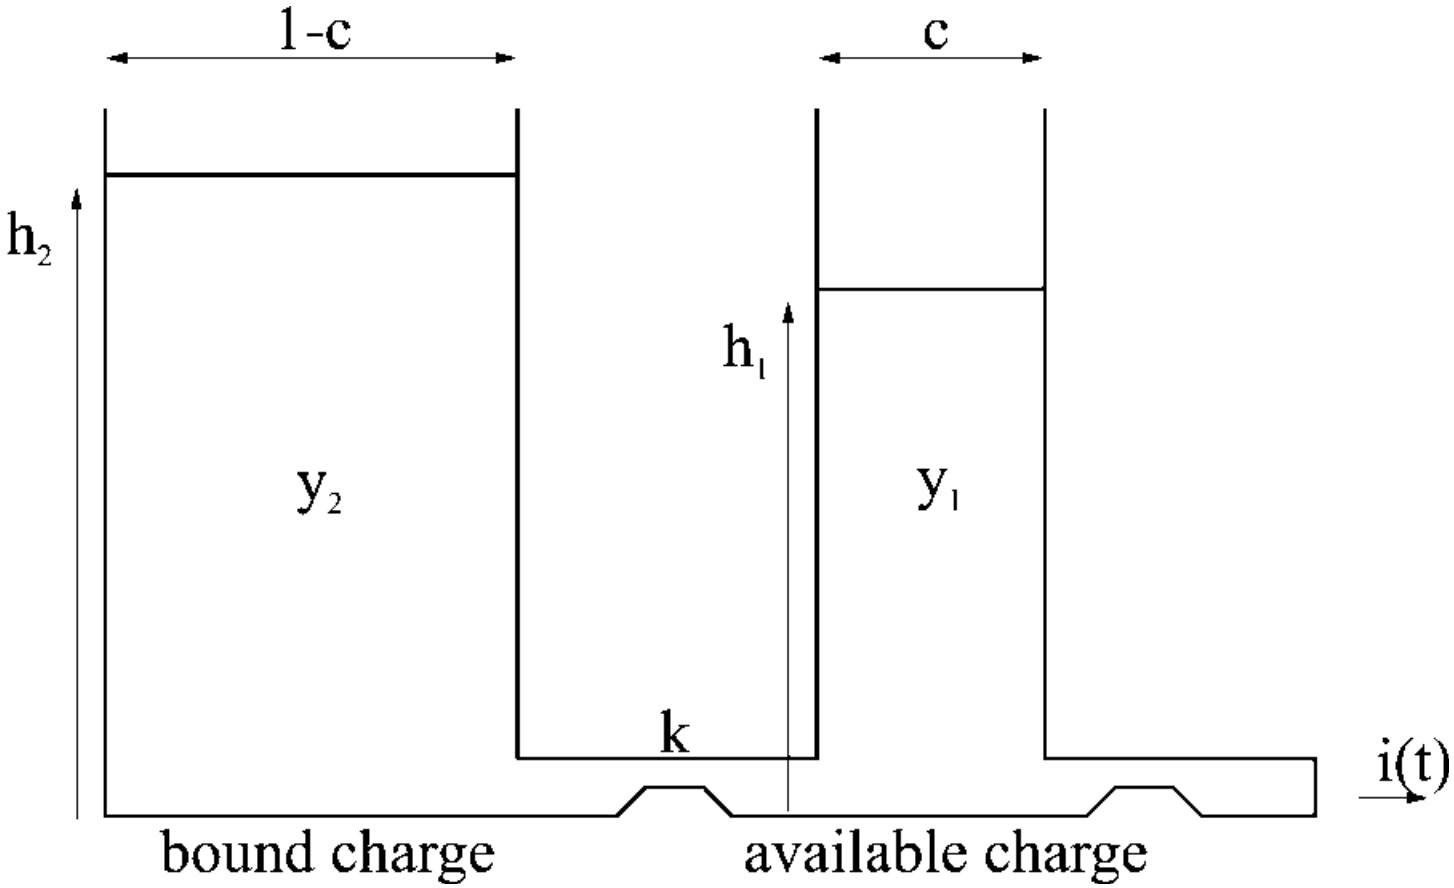
\includegraphics[width=\textwidth/2]{graphics/kibam.jpg}
	\caption{The two wells available(a) and bound(b)}
	\label{fig:kibam_wells}
\end{figure}

\begin{equation}\label{eq:y1}
y_1(t) = cCe^{-k't}+\frac{(y_0k'c-I)(1-e^{-k't})}{k'}-\frac{Ic(k't-1+e^{-k't})}{k'}
\end{equation}

\begin{equation}\label{eq:y2}
y_2(t) = (1-c)Ce^{-k't}+y_0(1-c)(1-e^{-k't})-\frac{I(1-c)(k't-1+e^{-k't})}{k'}
\end{equation}

C is capacity in Ah, e is Euler's number, k' is $k/c(1-c)$, k is a constant, t is time in hours, c is the ratio between available and bound charge, and I is the load current applied on the battery.

\Cref{table:t-KiBaM} shows the predictions when using \gls{kibam}.
Under constant load the results vary, and the the most precise predictions can be found when the amps are above 110 or below 20.
Interesting for variable loads, is that all of the predictions from \gls{kibam} underestimate compared to the measured values, some are fairly high as C7 underestimate by 40.31\%.

\begin{table}[H]
	\centering
	\scalebox{0.8}{
	\begin{tabular}{|l|lllll|llll|l|}
\hline
\multicolumn{6}{|c|}{Constant load} & \multicolumn{5}{c|}{Variable load} \\ \hline
\rowcolor[HTML]{EFEFEF} 
Test & \multicolumn{1}{l|}{\cellcolor[HTML]{EFEFEF}I, amps} & \multicolumn{1}{l|}{\cellcolor[HTML]{EFEFEF}Meas, min} & \multicolumn{1}{l|}{\cellcolor[HTML]{EFEFEF}KiBaM, min} & \multicolumn{1}{l|}{\cellcolor[HTML]{EFEFEF}$\Delta$T} & \%$\Delta$ & \multicolumn{1}{l|}{\cellcolor[HTML]{EFEFEF}Test} & \multicolumn{1}{l|}{\cellcolor[HTML]{EFEFEF}Meas, min} & \multicolumn{1}{l|}{\cellcolor[HTML]{EFEFEF}KiBaM, min} & $\Delta$T & \%$\Delta$ \\ \hline
T1 & 222.7 & 141.0 & 139.9 & -1.1 & -0.78\% & C1 & 54.5 & 36.3 & -18.2 & -33.39\% \\ \hline
\rowcolor[HTML]{EFEFEF} 
T2 & 204.5 & 156.6 & 156 & -0.6 & -0.38\% & C2 & 73.3 & 55.7 & -17.6 & -24.01\% \\ \hline
T3 & 108.3 & 307.8 & 331.4 & 23.6 & 7.67\% & C3 & 88.3 & 71.4 & -16.9 & -19.14\% \\ \hline
\rowcolor[HTML]{EFEFEF} 
T4 & 107.5 & 312.0 & 334.1 & 22.1 & 7.08\% & C4 & 136.0 & 123.6 & -12.4 & -9.12\% \\ \hline
T5 & 94.9 & 358.2 & 384 & 25.8 & 7.20\% & C5 & 182.7 & 175.7 & -7 & -3.83\% \\ \hline
\rowcolor[HTML]{EFEFEF} 
T6 & 84.3 & 397.2 & 437.5 & 40.3 & 10.15\% & C6 & 59.0 & 41.1 & -17.9 & -30.34\% \\ \hline
T7 & 75.5 & 448.2 & 493.3 & 45.1 & 10.06\% & C7 & 51.1 & 30.5 & -20.6 & -40.31\% \\ \hline
\rowcolor[HTML]{EFEFEF} 
T8 & 28.0 & 1248 & 1401 & 153 & 12.26\% & C8 & 55.0 & 38.1 & -16.9 & -30.73\% \\ \hline
T9 & 19.5 & 1818 & 2029 & 211 & 11.61\% & C9 & 54.9 & 34.8 & -20.1 & -36.61\% \\ \hline
\rowcolor[HTML]{EFEFEF} 
T10 & 3.0 & 12690 & 13417 & 727 & 5.73\% & C10 & 142.7 & 131.7 & -11 & -7.71\% \\ \hline
\end{tabular}}
	\caption{Comparison of actual measurements and predictions from the \gls{kibam}. Specification for the variable loads can be found in \cref{table:variable_loads_list}
	}
	\label{table:t-KiBaM}
\end{table}

Looking at all the results for the three battery models, it show that Peukert's model give overall better estimations for variable loads than Ideal and \gls{kibam}. 
But the advantage of using \gls{kibam} over Peukert's model under variable load, is that \gls{kibam} seems to always underestimate, which is attractive for our case.
Underestimating ensures that we will never run into a case where the prediction cause the actual system to run out of energy.
The Ideal is inferior to Peukert's and \gls{kibam} in almost all of the predictions, a summery of the three different battery models can be found below.
\begin{itemize}
	\item Ideal model - linear representation of the battery with no support of recovery effect
	\item Peukert model - non-linear representation of the battery with no support of recovery effect
	\item \gls{kibam} - abstract representation of the battery with support of recovery effect
\end{itemize}
\Gls{cora} can not use \gls{kibam} or Peukert's model because it only support cost with a linear rate and only natural numbers, the Ideal model will implemented in the \gls{cora} model.
